\documentclass[12pt]{article}
\usepackage{graphicx}
\usepackage{hyperref}
\usepackage[top=2.75in, left=1in, right=1in, bottom=0.25in]{geometry}
\usepackage[utf8]{inputenc}
\usepackage[english]{babel}
\usepackage{fancyhdr}
\usepackage[utf8]{inputenc}
\usepackage{listings}
\usepackage{color}
\usepackage[final]{pdfpages}
\usepackage{multirow}
\usepackage{array}
\usepackage{caption}
\usepackage{subcaption}


\definecolor{codegreen}{rgb}{0,0.6,0}
\definecolor{codegray}{rgb}{0.5,0.5,0.5}
\definecolor{codepurple}{rgb}{0.58,0,0.82}
\definecolor{backcolour}{rgb}{0.95,0.95,0.92} 
\lstdefinestyle{mystyle}{
    backgroundcolor=\color{backcolour},   
    commentstyle=\color{codegreen},
    keywordstyle=\color{magenta},
    numberstyle=\tiny\color{codegray},
    stringstyle=\color{codepurple},
    basicstyle=\footnotesize,
    breakatwhitespace=false,         
    breaklines=true,                 
    captionpos=b,                    
    keepspaces=true,                 
    numbers=left,                    
    numbersep=5pt,                  
    showspaces=false,                
    showstringspaces=false,
    showtabs=false,                  
    tabsize=2
} 
\lstset{style=mystyle}

\setlength{\parindent}{4em}
\setlength{\parskip}{1em}
\pagestyle{fancy}
\fancyhf{}
\rhead{Assignment 7}
\lhead{Huan Huang}
\renewcommand{\headrulewidth}{0.4pt}
\renewcommand{\footrulewidth}{0.4pt}
\rfoot{Page \thepage}


\begin{document}
\begin{titlepage}
	\begin{center}
	\Huge{Web Science cs532-s16}\\
	[0.25in]
	\textsc{\Large Assignment 7 Report}\\
	\textsc{\normalsize Dr. Michael L. Nelson}\\
	[4.25in]
	\textsc{\normalsize By: Huan Huang}\\
	\large 03/31/2016\\
	
	
	\end{center}
\end{titlepage}
\newpage

\newgeometry{margin=1in}

\section*{Assignment Description}

The goal of this project is to use the basic recommendation principles
we have learned for user-collected data. You will modify the code
given to you which performs movie recommendations from the MovieLense
data sets.

The MovieLense data sets were collected by the GroupLens Research
Project at the University of Minnesota during the seven-month period
from September 19th, 1997 through April 22nd, 1998.  We are using the 
``100k dataset"; available for download from:
http:\/\/grouplens.org\/datasets\/movielens\/100k\/

\noindent
There are three files which we will use:

\noindent
1.  u.data: 100,000 ratings by 943 users on 1,682 movies. Each
user has rated at least 20 movies. Users and items are numbered
consecutively from 1. The data is randomly ordered. This is a tab
separated list of 

\begin{verbatim}
user id | item id | rating | timestamp
\end{verbatim}

\noindent
The time stamps are unix seconds since 1/1/1970 UTC.

\noindent
Example:

\begin{verbatim}
196     242     3       881250949
186     302     3       891717742
22      377     1       878887116
244     51      2       880606923
166     346     1       886397596
298     474     4       884182806
115     265     2       881171488
\end{verbatim}

\noindent
2.  u.item: Information about the 1,682 movies. This is a tab
separated list of

\begin{verbatim}
movie id | movie title | release date | video release date | IMDb URL | 
unknown | Action | Adventure | Animation |Children's | Comedy | Crime | 
Documentary | Drama | Fantasy | Film-Noir | Horror | Musical | Mystery | 
Romance | Sci-Fi | Thriller | War | Western |
\end{verbatim}

The last 19 fields are the genres, a 1 indicates the movie is of
that genre, a 0 indicates it is not; movies can be in several genres
at once. The movie ids are the ones used in the u.data data set.
\newpage

\noindent
Example:

\begin{verbatim}
161|Top Gun (1986)|01-Jan-1986||http://us.imdb.com/M/title-exact?Top
%20Gun%20(1986)|0|1|0|0|0|0|0|0|0|0|0|0|0|0|1|0|0|0|0 

162|On Golden Pond (1981)|01-Jan-1981||http://us.imdb.com/M/title-
exact?On%20Golden%20Pond%20(1981)|0|0|0|0|0|0|0|0|1|0|0|0|0|0|0|0|0|0|0 

163|Return of the Pink Panther, The (1974)|01-Jan-1974||http://
us.imdb.com/M/title-exact?Return%20of%20the%20Pink%20Panther,%20The
%20(1974)|0|0|0|0|0|1|0|0|0|0|0|0|0|0| 0|0|0|0|0
\end{verbatim}

\noindent
3.  u.user: Demographic information about the users. This is a tab
separated list of:

\begin{verbatim}
user id | age | gender | occupation | zip code
\end{verbatim}

\noindent
The user ids are the ones used in the u.data data set.

\noindent
Example:

\begin{verbatim}
1|24|M|technician|85711 
2|53|F|other|94043 
3|23|M|writer|32067 
4|24|M|technician|43537 
5|33|F|other|15213
\end{verbatim}

The code for reading from the u.data and u.item files and creating
recommendations is described in the book Programming Collective
Intelligence.  Feel free to modify the PCI code to answer the 
following questions.

\section*{Problem 1}

\noindent
Find 3 users who are closest to you in terms of age, 
gender, and occupation.  For each of those 3 users:

\noindent
- what are their top 3 favorite films?
- bottom 3 least favorite films?

\noindent
Based on the movie values in those 6 tables (3 users X (favorite +
least)), choose a user that you feel is most like you.  Feel 
free to note any outliers (e.g., ``I mostly identify with user 123,
except I did not like ``Ghost'' at ll").  

\noindent
This user is the ``substitute you".  


\subsection*{Answer}
To solve this problem, I first downloaded the 3 files from the link provided in the assignment description above. Then I proceed to write a code to identify the users who are closest resemblance of me, based on the age, gender, and occupation in the u.user file. Below are all of the candidates who fit the 3 criteria.

\begin{figure}[h]
\centering
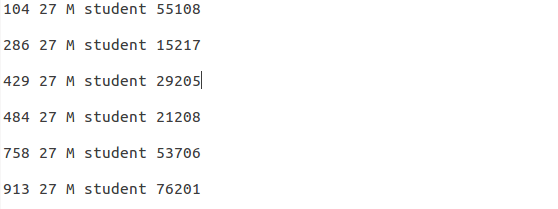
\includegraphics[width=6.5in]{inisub.png}
\caption{The initial candidates to be the substitute me}
\end{figure}

\lstinputlisting[language=python]{substitute.py}

From this list, I hand picked 3 individuals for the next stage. The 3 users I picked are 286, 429, and 484.
 
\lstinputlisting[language=python]{substitute.txt}

Now, for each of the 3 user, I access all of his movie ratings, if the rating is 5, the movie id is appended to an array; if the rating is 1, the movie id is appended to another array. Then I open the u.item file to get the movie titles. I only print out 3 items in each of the array, this gives me the 3 favorite and 3 least favorite movies of the 3 users.
\newpage

\begin{figure}[h]
\centering
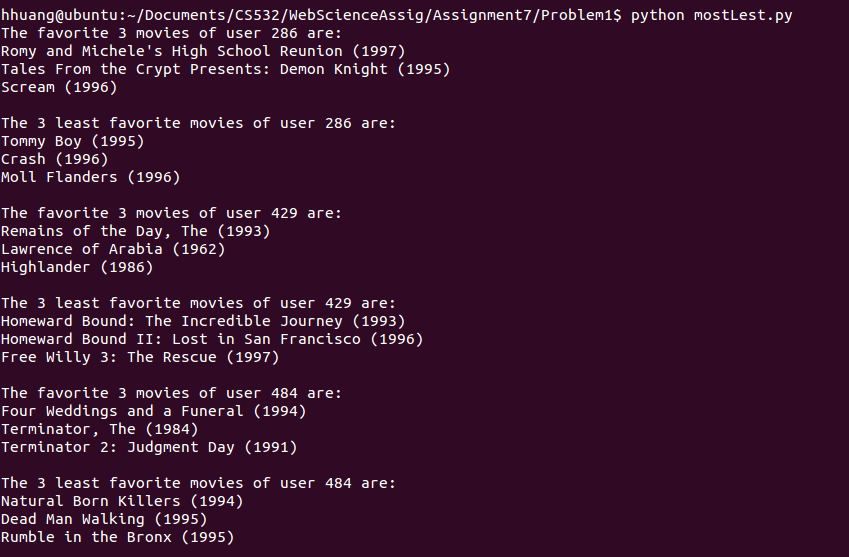
\includegraphics[width=6.5in]{mostleast.png}
\caption{The 3 most and least favorite movies of the 3 users}
\end{figure}

Based on the favorite and least favorite movies of the 3 users, I can clearly tell that user 484 is much closer to me in term of movie preference. Because I love The Terminator I and II. Although, I have not watched any other movies in his favorite or least favorite movie list, he is still the closest match out of the 3 candidates.
\newpage

\section*{Problem 2}

Which 5 users are most correlated to the substitute you? Which
5 users are least correlated (i.e., negative correlation)?

\subsection*{Answer}

Let me be clear at this point, for this problem, and the rest of the problems in this assignment, I copied and modified code from recommendations.py provided by the book Programming Collective Intelligence. They have a github account where all of their code are available there, here is the link for recommendations.py: \url{://github.com/cataska/programming-collective-intelligence-code/blob/master/chapter2/recommendations.py}. 

I applied 3 functions from the recommendations.py file, the loadMovieLens() which loop through every line in u.item file and store the movie id and title into the a dictionary, then loops through u.data file to attach each movie and its ratings to its rater, the result is stored in dictionary prefs\{\}. Then the prefs will be passed to function topMatches() along with the user id ``484" to find the most and least correlated users of user 484. The function topMatches() will call another function sim\_pearson() to use Pearson method of calculating correlation coefficient between user 484 and other users based on their ratings. 

\begin{figure}[h]
\centering
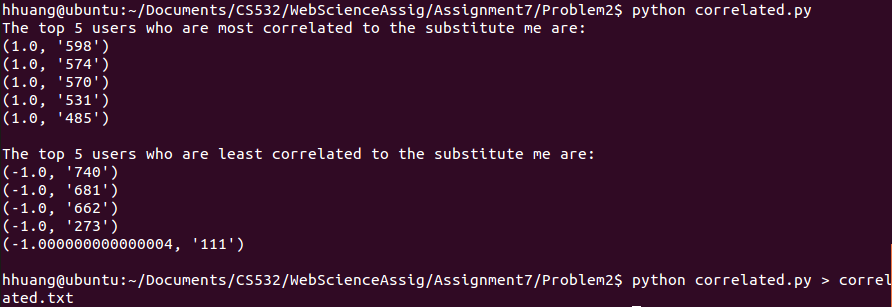
\includegraphics[width=6.5in]{correlated.png}
\caption{The 5 most and least correlated users to the substitute me}
\end{figure}

\lstinputlisting[language=python]{correlated.py}

\section*{Problem 3}

Compute ratings for all the films that the substitute you
hasn't seen.  Provide a list of the top 5 recommendations for films
that the substitute you should see.  Provide a list of the bottom
5 recommendations (i.e., films the substitute you is almost certain
to hate).

\subsection*{Answer}

For this problem, I used 3 functions from recommendations.py: use loadMovieLens() to get the necessary data, sim\_pearson() to calculate the correlation coefficient of user 484 and other users, and getRecommendations() to calculate the recommendations for user 484 based on the result from sim\_pearson() function. 

\begin{figure}[h]
\centering
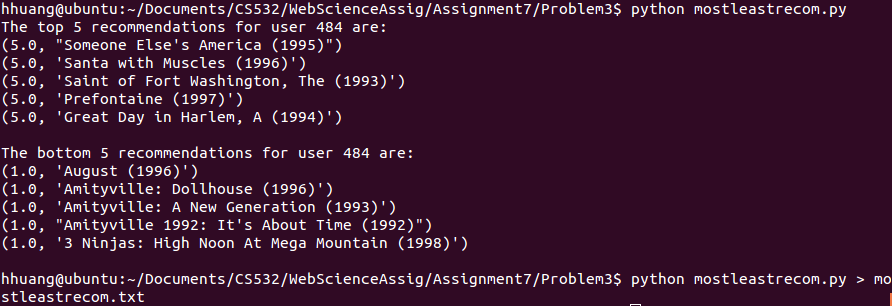
\includegraphics[width=6.5in]{mostleastrecom.png}
\caption{The 5 most and least recommended films for the substitute me}
\end{figure}

\lstinputlisting[language=python]{mostleastrecom.py}

\section*{Problem 4}

Choose your (the real you, not the substitute you) favorite and
least favorite film from the data.  For each film, generate a list
of the top 5 most correlated and bottom 5 least correlated films.
Based on your knowledge of the resulting films, do you agree with
the results?  In other words, do you personally like / dislike
the resulting films?

\subsection*{Answer}

My favorite movie in this list is ``The Godfather: Part II(1974)" and my least favorite movie is ``Turbo: A Power Rangers Movie (1997)". The method to solve this problem is similar to problem 2, but this time, I have to use the function transformPrefs() to remap the dictionary perfs\{\}. As a result, when the function topMatches() calls function sim\_pearson(), it is passing a set of data that enables sim\_pearson() to calculate the correlation of movies based on their ratings. 

\begin{figure}[h]
\centering
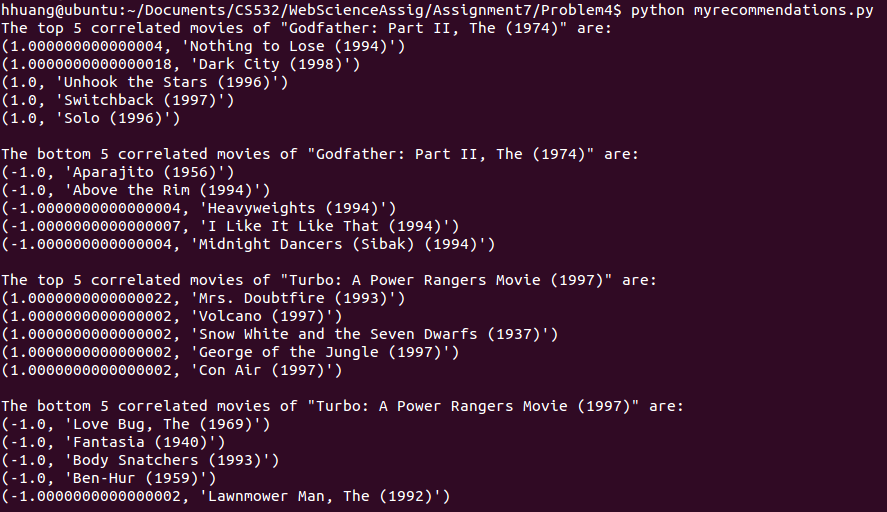
\includegraphics[width=6.5in]{myrecommendations.png}
\caption{The 5 most and least correlated films for my most and least favorite movies}
\end{figure}

It is hard to determine the accuracy of the recommendations based on this result. Because I have not watched any of the most and least correlated movies for Godfather II, therefore, I can't really agree or disagree with the results of my favorite movie. However, I do agree with the list for my least favorite movie. The top correlated films of ``Turbo: A Power Rangers Movie (1997)" are all horrible movies that I have no interest in whatsoever. 
\pagebreak

\lstinputlisting[language=python]{myrecommendations.py}


\end{document}